\documentclass[a4paper]{article}

\usepackage[english]{babel}
\usepackage[utf8x]{inputenc}
\usepackage{amsmath}
\usepackage{graphicx}
\usepackage[margin=0.5in]{geometry}
\usepackage{cleveref}
\title{Project 1 Analysis}
\begin{document}
\maketitle
Turns out I was plotting my exact solution wrong... This took me a while to realize. \Cref{fig:highdt}.
\begin{figure}
    \centering
    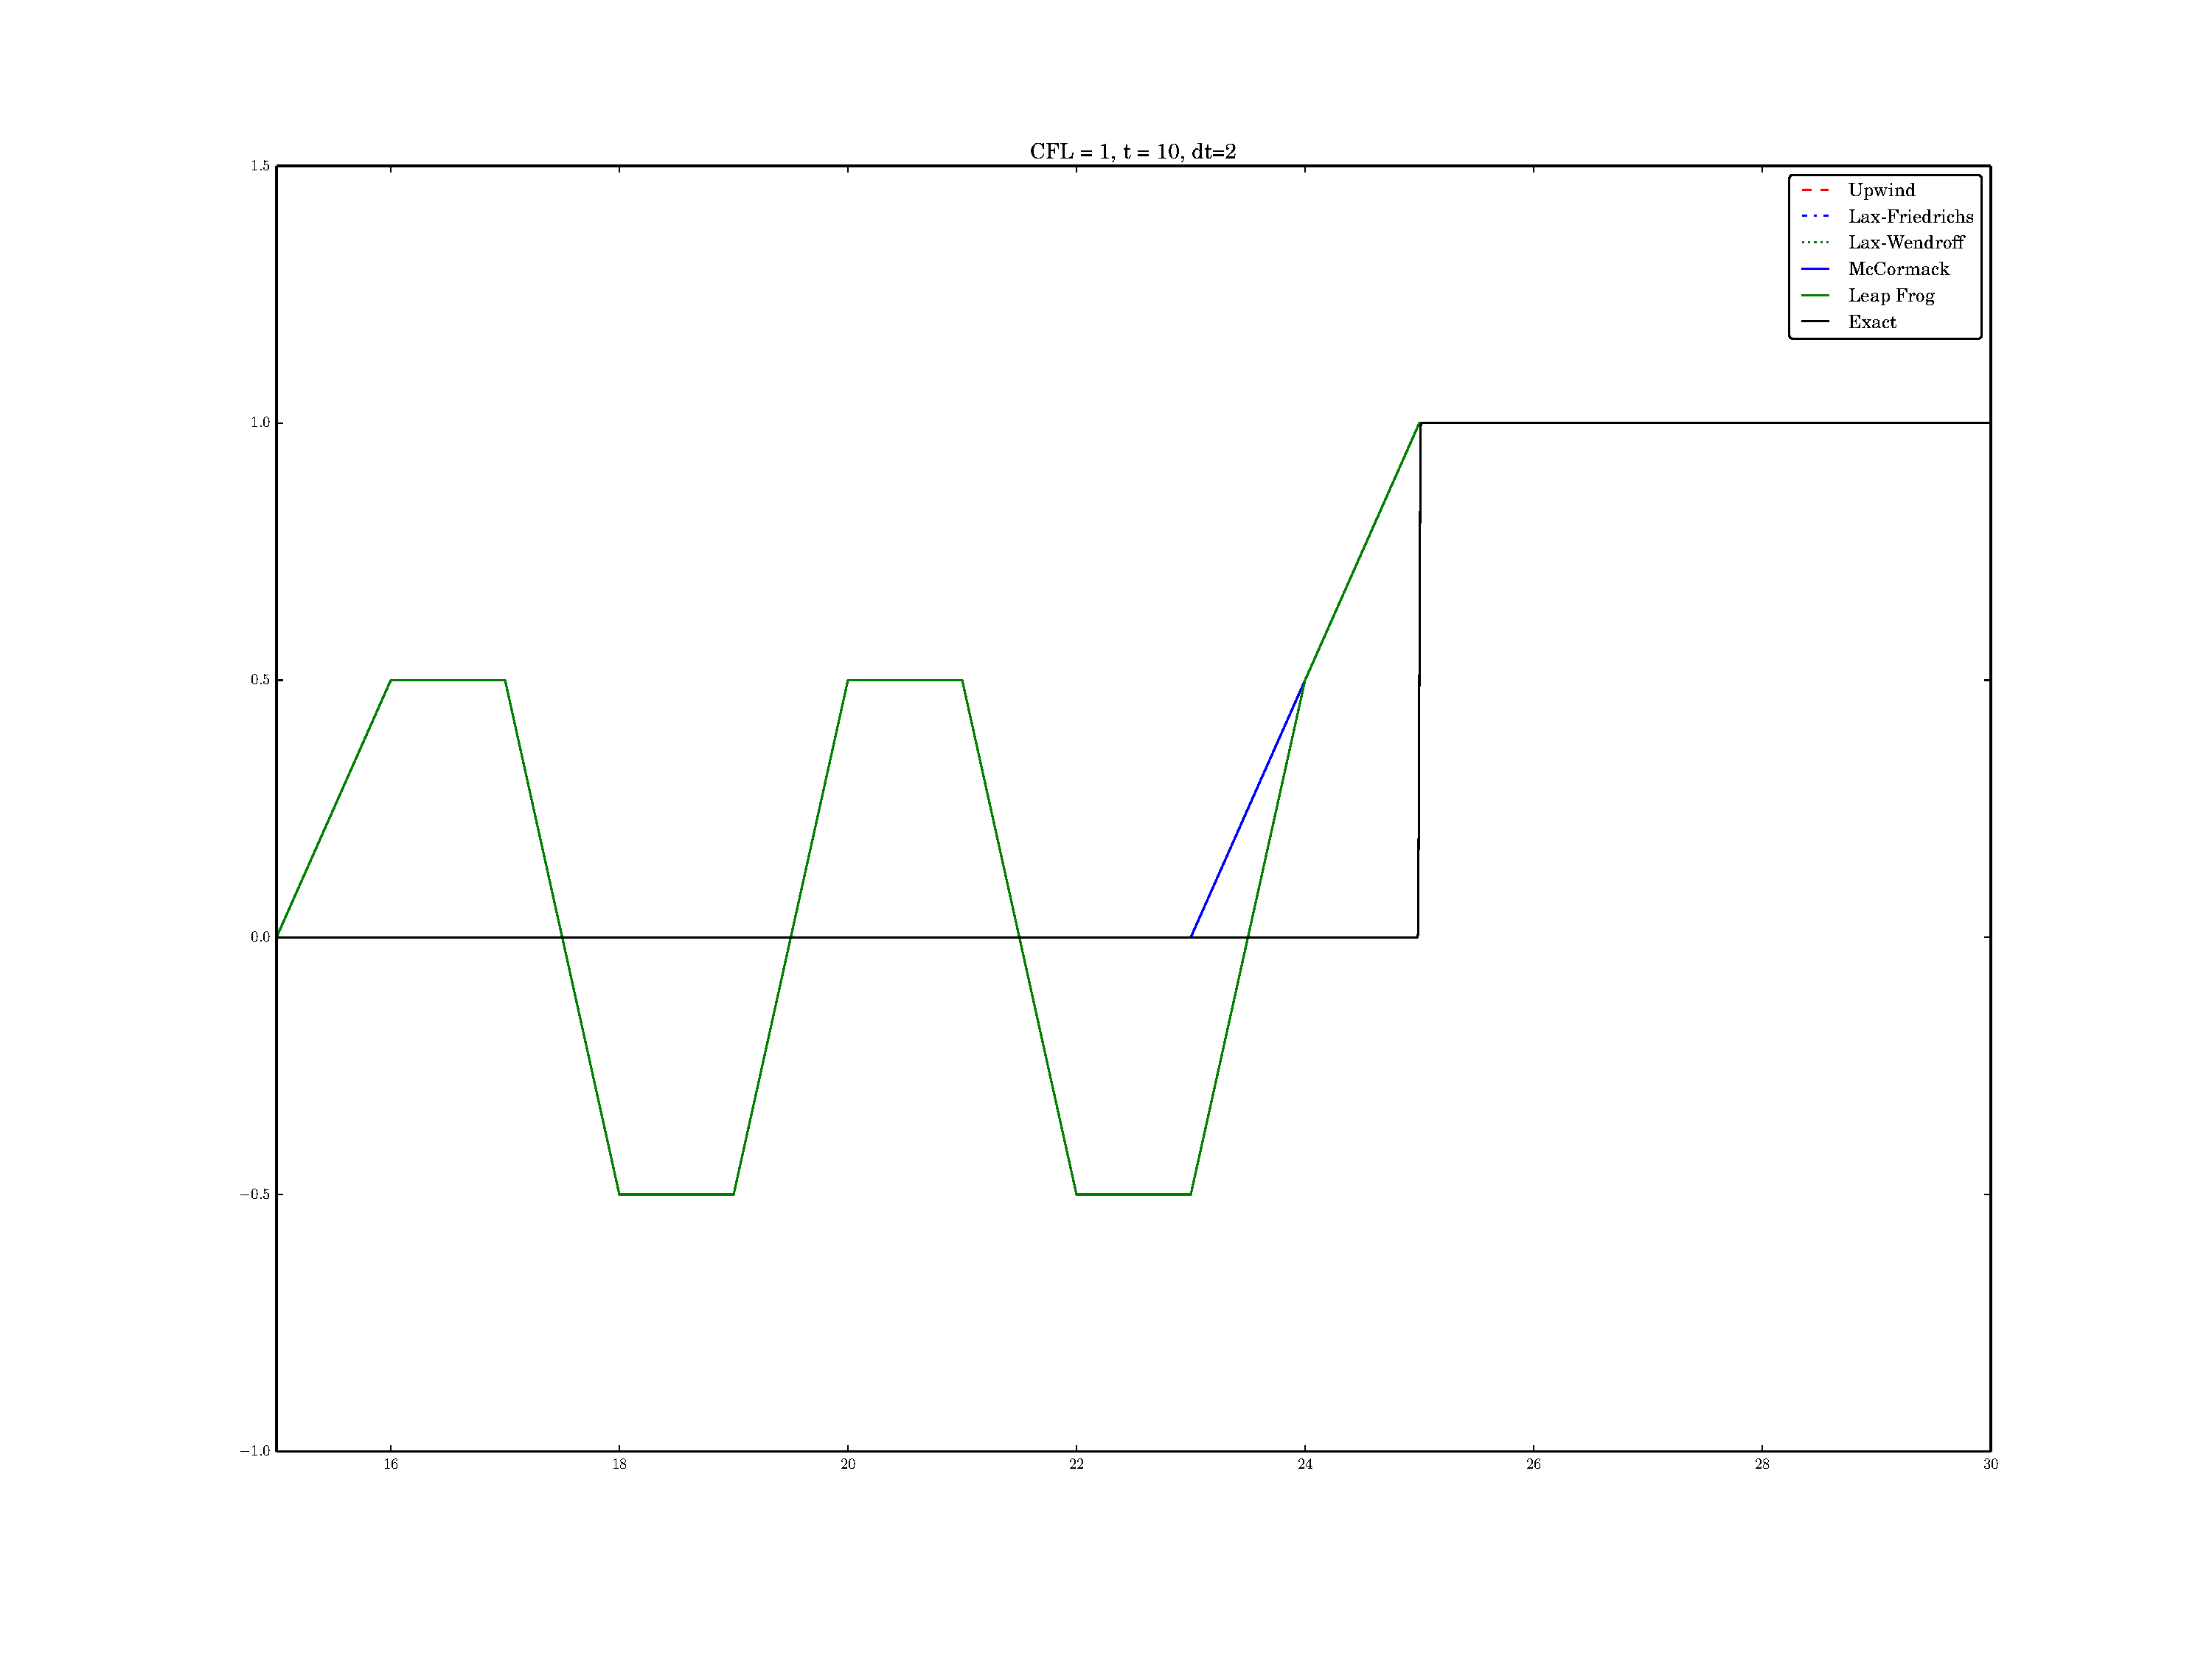
\includegraphics[width=1.0\textwidth]{highdt.pdf}
    \caption{High $\Delta t$}\label{fig:highdt}
\end{figure}

I know $CFL = \nu = 1$ is the limit of stability for these schemes. I tried with CFL = 1.05 and all the schemes start to blow up!

Now, I found it was weird that Lax-Wendroff, Upwind and Lax-Friedrichs gave exactly the same results, so I looked at the TE for these schemes. I didn't derive the Truncation Error for Leap Frog or McCormack.

\section{Truncation Error}

Performing a Taylor expansion on the Upwind, Lax-Friedrichs and Lax-Wendroff schemes leads to the truncation error. Moreover, replacing time derivatives with spatial derivatives allows us to notice the artificial dissipation and dispersion introduced by these schemes -- dissipation in the case of Upwind and Lax-Friedrichs, dispersion in Lax-Wendroff.

If we rearrange such that the dissipation/dispersion terms are functions of $\nu$, we can notice that these terms vanish for $\nu = 1$. \textbf{This explains why Upwind, Lax-Friedrichs, Lax-Wendroff have the same profile for $\nu = 1$}.

Moreover, in the case that $\nu > 1$, the dissipation is \emph{negative}, i.e. the dissipation turns into an \emph{amplification}. As for dispersion, the artificial dispersive term is this:
\begin{equation}
\label{eq:dispersion}
\frac{A\Delta x^2}{6}(\nu^2 - 1)u_{xxx}
\end{equation}
which is \emph{negative} for $\nu < 1$ and becomes positive for $\nu > 1$. I'm not sure what this physically means, but it clearly makes the solution unstable.

Thus, for $\nu = 1$, the linear advection equation is supposedly solved exactly as only the higher order derivative terms are left. However, this is only true for low enough $\Delta t$ and $\Delta x$, especially in this case where exact solution is almost discontinuous. So, do we recover the exact solution for low $\Delta t, \Delta x$?

\section{Lowering $\Delta t, \Delta x$}
Consequently, I also tried decreasing both $\Delta t$ and $\Delta x$, but such that I keep $\nu = 1$. In this case, I do recover the exact solution. See~\Cref{fig:lowdt}.
\begin{figure}
    \centering
    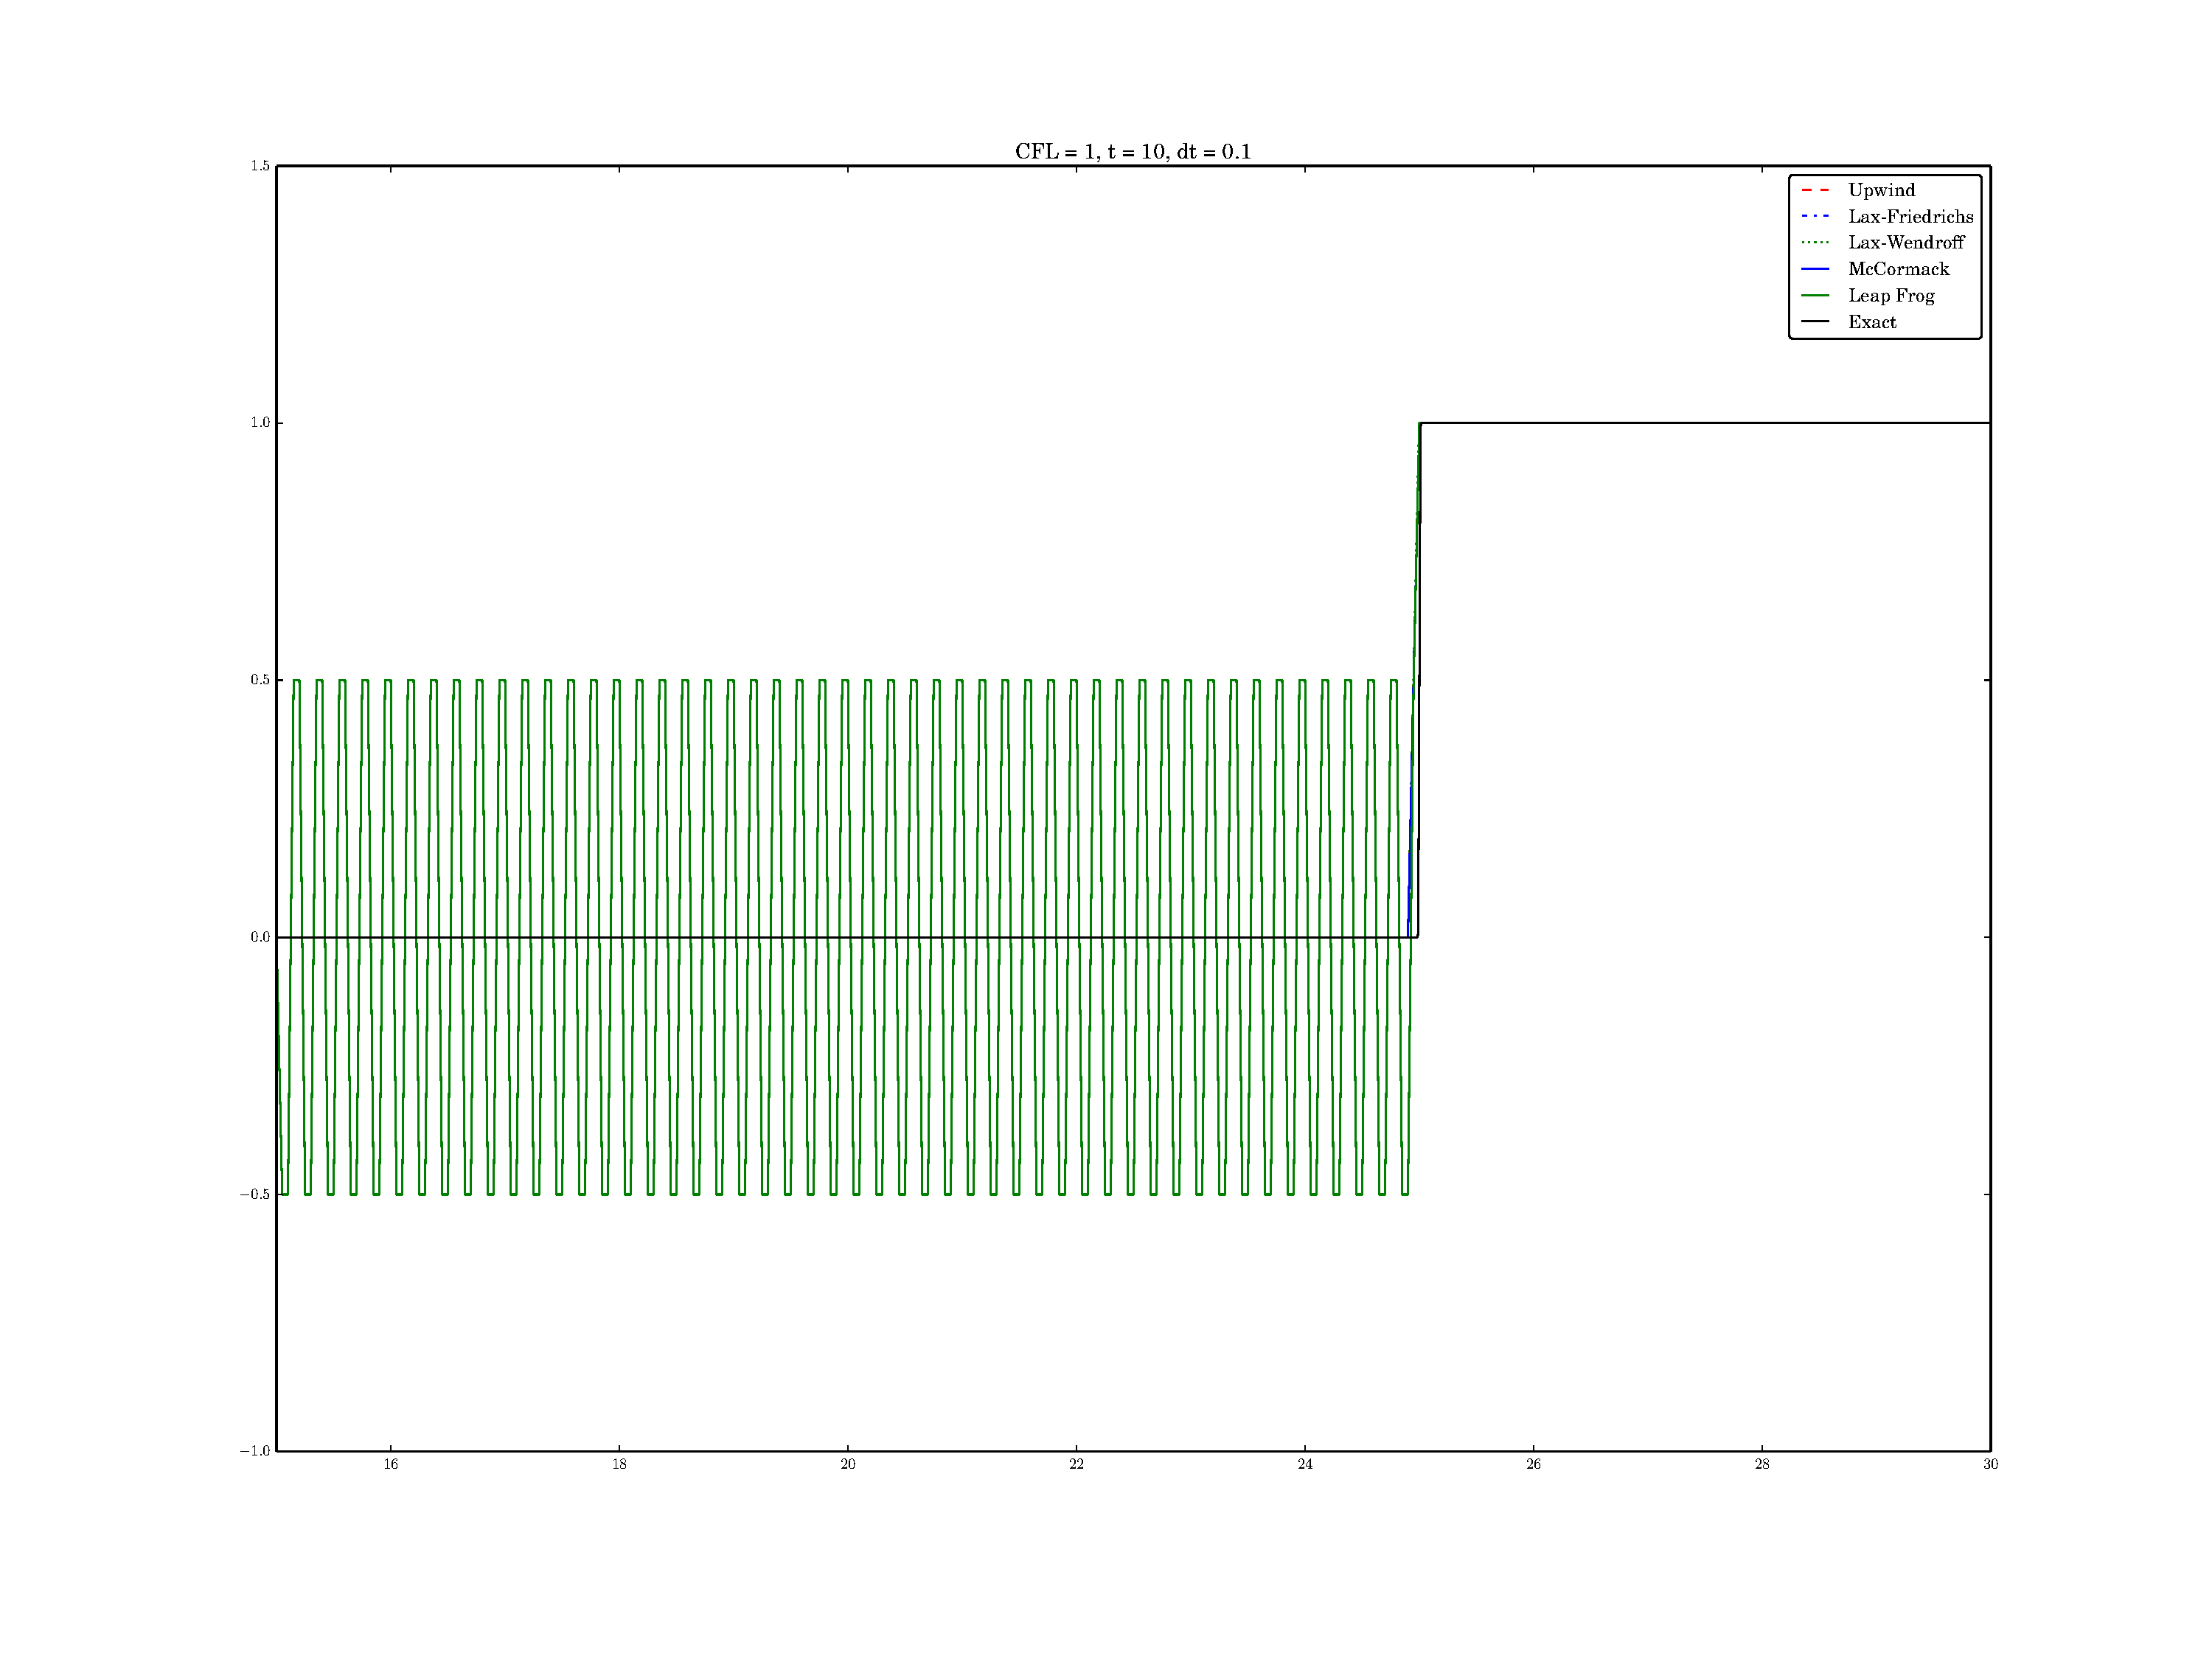
\includegraphics[width=1.0\textwidth]{lowdt.pdf}
    \caption{Low $\Delta t$. Results for Lax* and Upwind are exact.}\label{fig:lowdt}
\end{figure}

\section{Leap Frog and McCormack?}
I re-checked my code for Leap Frog and McCormack multiple times, but I believe it to be correct since the results for a $\nu = 0.25$, as in ~\Cref{fig:cfl_025}, make sense for these two schemes. However, doing a Taylor expansion of the Leap frog scheme gives me:
\begin{equation}
(u_t + Au_x) = \frac{A\Delta x^2}{6}(\nu^2 - 1)u_{xxx} + ...
\end{equation}
which is the same dispersive term as in Lax-Wendroff, so I'm puzzled.

\begin{figure}
    \centering
    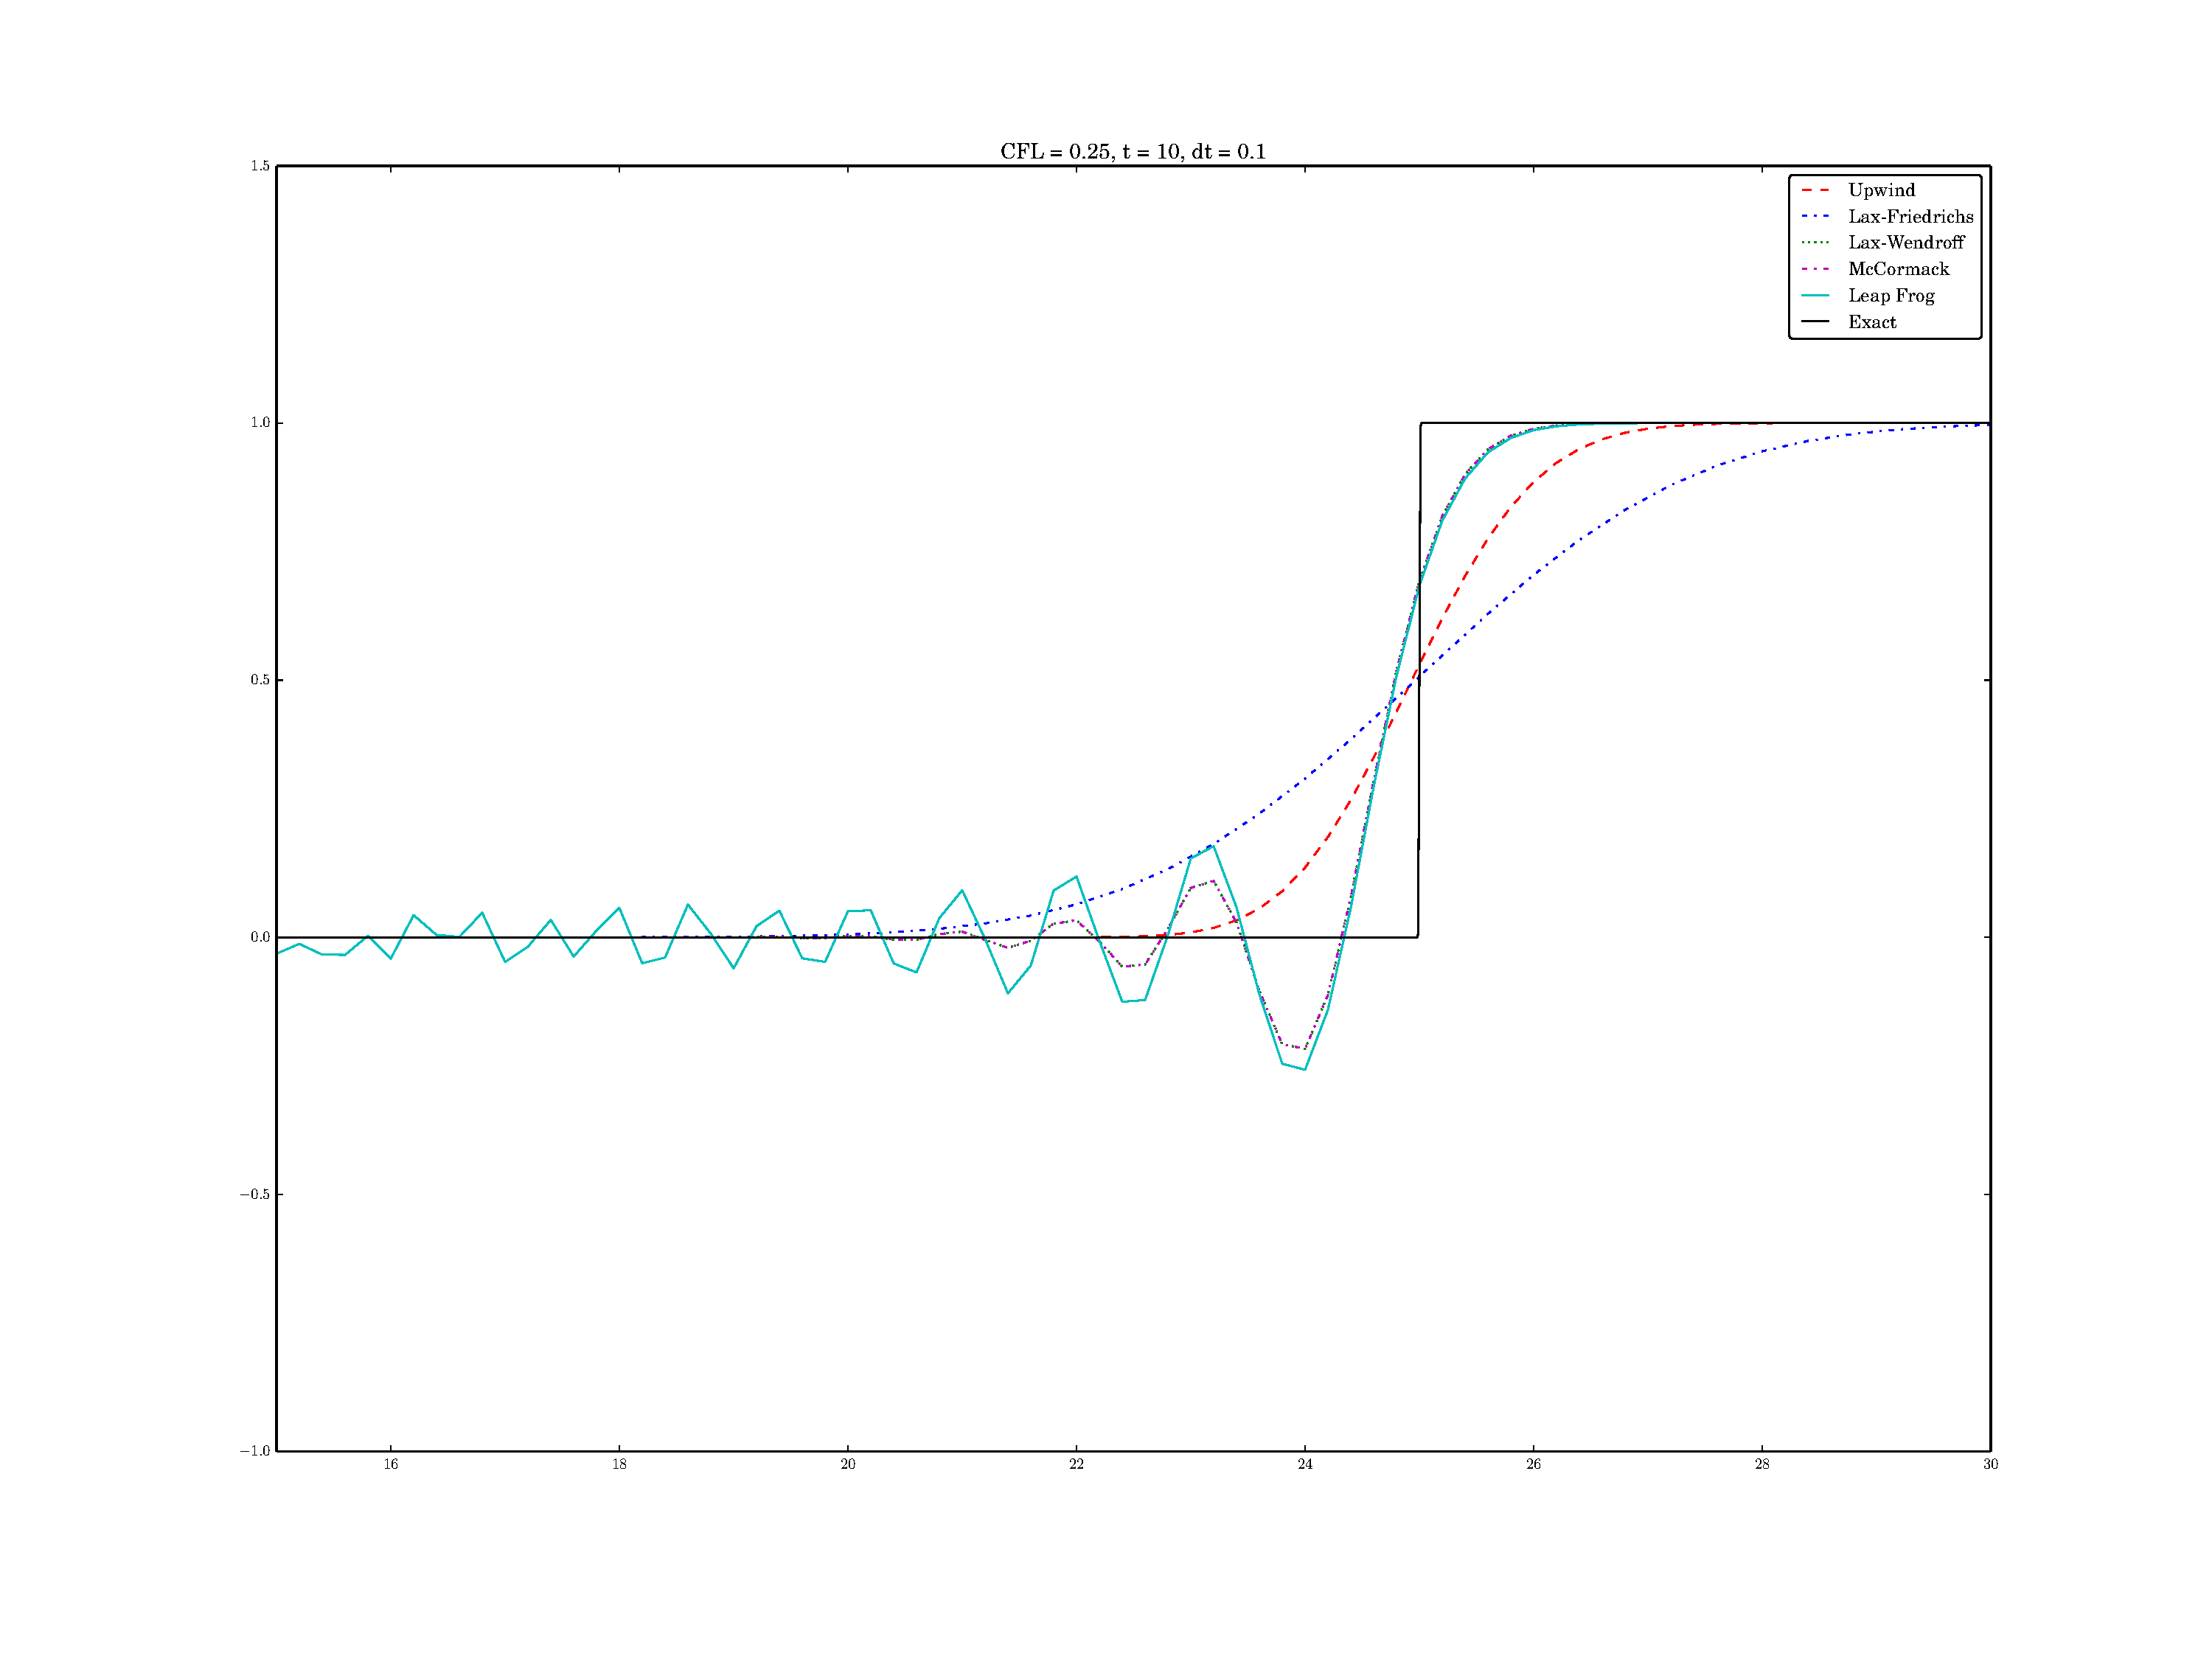
\includegraphics[width=1.0\textwidth]{cfl_025.pdf}
    \caption{Lower $\nu$. Results for Leap Frog and McCormack are realistic.}\label{fig:cfl_025}
\end{figure}


\end{document}